\documentclass[a4paper,10pt]{article}

\usepackage[T1]{fontenc}
\usepackage[latin1]{inputenc}
\usepackage{amsmath}
\usepackage{amssymb}
\usepackage{graphicx}
\usepackage{fancybox}
\usepackage{geometry}

%opening
\title{Direction Finding as relevant for the\\ STEREO/SWAVES experiment}
\author{Thomas Oswald}

\begin{document}

\maketitle

\begin{abstract}
Direction Finding is the process of finding the 6 parameters that define an electromagnetic (EM) wave. It will be a vital part of the STEREO mission, conducted by NASA, to be launched in spring 2006. In this report, I will outline the methods and equation systems available to date, in regard to the the STEREO/SWAVES experiment.
\end{abstract}

\section{Introduction}

\paragraph*{}
STEREO is a space mission, conducted by NASA, to be launched in spring 2006. The mission consists of two space probes which will enter a heliocentric orbit. One spacecraft will orbit sun ahead of the earth, the other behind.

\paragraph*{}
The scientific goal of the mission is to increase our knowledge of the physics of our solar system, especially:\\

\begin{itemize}
\item  Understanding the causes and mechanisms of CME initiation
\item Characterize the propagation of CMEs through the heliosphere
\item Discover the mechanism and sites of energetic particle acceleration in the low corona and the interplanetary medium
\item Develop a 3D time dependent model of the magnetic topology, temperature, density and velocity structure of the ambient solar wind.
\end{itemize}

 \paragraph*{}
Among several other experiments, one particular important is STEREO WAVES (SWAVES). This experiment is designed to track interplanetary radio bursts and trace the generation and evolution of radio disturbances from the sun to earth orbit and beyond. Each spacecraft has three, nearly orthogonal, antennas. With this configuration, it is possible to perform direction finding (DF) to find the direction of the origin of the received radiation and information about its polarization. When both spacecraft receive radiation from the same source at the same time, the actual location of the source can be pinpointed by the method of triangulation.

\paragraph*{}
SWAVES uses 3, nearly orthogonal, antennas to receive EM radiation in the frequency range of 16MHz. Direction finding will be performed in the lower part of this spectrum, up to a frequency of 2MHz. The output of the receiver is a combination of auto and cross correlation parameters, depending on the mode in use. All different combinations of correlation parameters can be obtained. The spacecraft will maintain a fixed orientation in space, a fact that has to be considered, when doing the analysis of possible methods of direction finding.
\newpage
\section{DF Basics}
Figure \ref{fig_coordinate_frame_DF} defines the symbols and coordinate system which will be used throughout this section.\\

\begin{center}
\begin{figure}
  % Requires \usepackage{graphicx}
  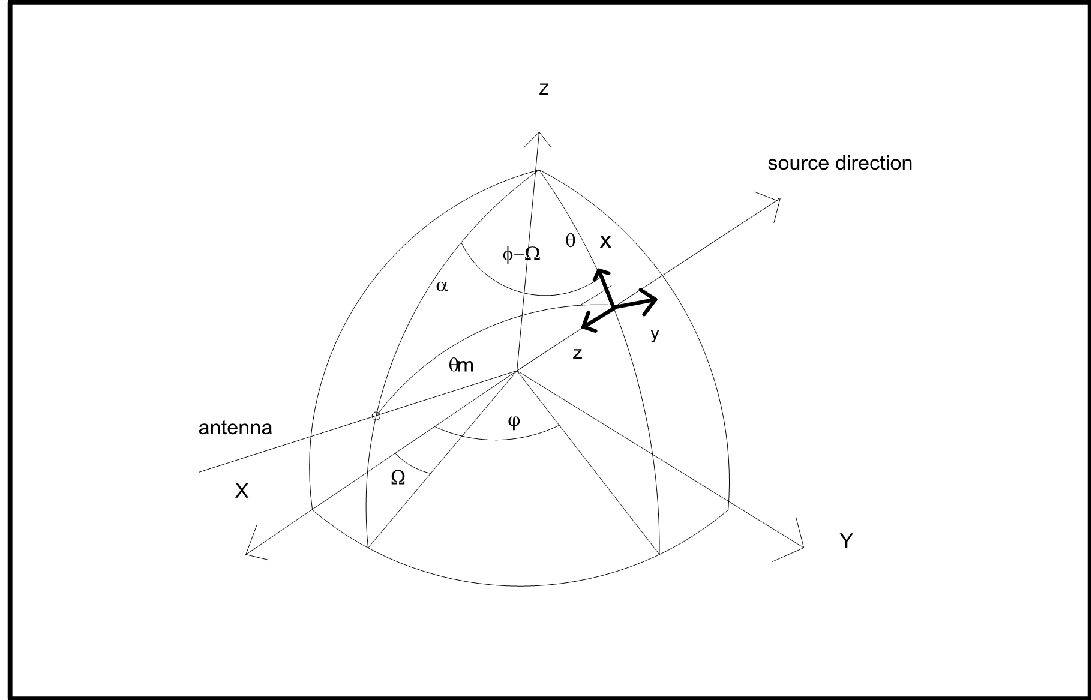
\includegraphics[width=12cm]{df_coordinate_system.eps}\\
  \caption{Coordinate Frame}\label{fig_coordinate_frame_DF}
\end{figure}\end{center}


X, Y and Z define the spacecraft centered orthogonal cartesian coordinate system, while x,y and z define the coordinate system of the incident electromagnetic wave. The wave vector $\textbf{k}$ is points in the positive z-axis, so the equation of the electric field of the wave is
\begin{equation}
\textbf{E}=\textbf{E}_0 e^{i(\textbf{k} \cdot \textbf{r} - \omega t)}
\end{equation}

\paragraph*{}
The electric field is the sum of the components in x and y direction. There is no component in the z direction.
\begin{eqnarray}
\textbf{E}&=&E_x\textbf{e}_x + E_y\textbf{e}_y\\
E_x&=&E_{0,x} e^{i(kz - \omega t)} \label{Ex} \\
E_y&=&E_{0,y} e^{i(kz - \omega t - \delta)} \label{Ey}
\end{eqnarray}
\paragraph*{}
$\delta$ is the phase shift between the x and y components of the E-field. The direction of the incident wave is defined by the angles $\vartheta$ and $\varphi$, the effective height vector points to the direction that is defined by the angles $\alpha$ and $\Omega$.
\paragraph*{}
The 4 Stokes Parameter define the polarization of the wave. They can be written in the following form:
\begin{equation}
S_0=I= \left\langle E_{0,x}^2\right\rangle +\left\langle E_{0,y}^2\right\rangle
\end{equation}
\begin{equation}
S_1=Q=\left\langle E_{0,x}^2\right\rangle-\left\langle E_{0,y}^2\right\rangle
\end{equation}
\begin{equation}
S_2=U=\left\langle2E_{0,x} E_{0,y} \cos \delta \right\rangle
\end{equation}
\begin{equation}
S_3=V=\left\langle2E_{0,x} E_{0,y} \sin\delta\right\rangle
\end{equation}
\\
\paragraph*{}
The Stokes Parameters are more useful in normalized form.
\begin{eqnarray}
\frac{S_0}{2\eta_0} = \hat{I} &=& \frac{\left\langle E_{0,x}^2\right\rangle +\left\langle E_{0,y}^2\right\rangle}{2\eta_0} \label{norm_stokes_1}
\\
\frac{S_1}{S_0}=\hat{Q}&=&\frac{\left\langle E_{0,x}^2\right\rangle-\left\langle E_{0,y}^2\right\rangle}{\left\langle E_{0,x}^2\right\rangle +\left\langle E_{0,y}^2\right\rangle}\label{norm_stokes_2}
\\
\frac{S_2}{S_0}=\hat{U}&=&\frac{\left\langle2E_{0,x} E_{0,y} \cos\delta\right\rangle}{\left\langle E_{0,x}^2\right\rangle +\left\langle E_{0,y}^2\right\rangle}\label{norm_stokes_3}
\\
\frac{S_3}{S_0}=\hat{V}&=&\frac{\left\langle2E_{0,x} E_{0,y} \sin\delta\right\rangle}{\left\langle E_{0,x}^2\right\rangle +\left\langle E_{0,y}^2\right\rangle}\label{norm_stokes_4}
\end{eqnarray}
\paragraph*{}
The output values of the measurements are the auto- and crosscorrelation parameters. For two antennas X and Z, they would be\\
\\
\begin{center}
\begin{tabular}{c}
$\left\langle V_X V_X^* \right\rangle $  \\
$\left\langle V_Z V_Z^* \right\rangle $  \\
$Re\left\langle V_X V_Z^* \right\rangle $  \\
$Im\left\langle V_X V_Z^* \right\rangle $  \\
\end{tabular}
\end{center}

\paragraph*{}
$V_i$ is the voltage induced in antenna i and the star means the complex conjugate. The angular brackets mean the mean value. In general, for a complex function $C(t)$,
\begin{equation}
\left\langle CC^* \right\rangle = \frac{1}{T}\int_0^T CC^* dt
\end{equation}

\paragraph*{}
This equation gives only a good result, if T is large in relation to the period of the EM wave. So the next step is to find a formula for V. The basic equation, upon which the method is built, is
\begin{equation}
V=\textbf{h}_{eff}\cdot \textbf{E}
\end{equation}
\paragraph*{}
$\textbf{h}_{eff}$ is the effective length vector. The radiation pattern of the antenna is, as if it was a sole monopole that points in the direction of $\textbf{h}_{eff}$ and with the same length. In general, the effective length vector depends on the frequency and direction of the incoming wave, but these dependencies are being neglected during this work, because at the time of writing, direction finding is only considered to be possible at low frequencies, where this is not the case. At wavelengths that are large in relation to the receiving antenna, $h_{eff}$ can be expected to be approximately half of the physical antenna.
\paragraph*{}
When written in component form, one can write
\begin{equation}
V=h_{eff,x} E_x + h_{eff,y} E_y \footnote{The coordinate frame is defined in a way that the electric field has no z-component}
\end{equation}
\paragraph*{}
After substituting equations (\ref{Ex}) and (\ref{Ey})...
\begin{equation}
V=h_{eff,x} E_{0,x} e^{i(kz - \omega t)}  + h_{eff,y} E_{0,y} e^{i(kz - \omega t - \delta)}
\end{equation}
\paragraph*{}
If the antenna is located at z=0 and short in relation to the wavelength, it can be simplified.
\begin{equation}
V=h_{eff,x} E_{0,x} e^{i(\omega t)}  + h_{eff,y} E_{0,y} e^{i(\omega t - \delta)} \label{V}
\end{equation}
\paragraph*{}
Hence, the next step is to find the x and y components of $\textbf{h}_{eff}$. By using the unit vector in the direction of $\textbf{h}_{eff}$, one can write

\begin{equation}
\textbf{h}_{eff} = h_{eff}\left[ \begin{array}{c}
\sin \alpha \cos \Omega\\
\sin \alpha \sin \Omega\\
\cos \alpha
\end{array}  \right]
\end{equation}

\paragraph*{}
The unit vectors of the spherical coordinate system are
\begin{eqnarray}
\textbf{e}_r &=& \left[ \begin{array}{c}
\sin \theta \cos \varphi\\
\sin \theta \sin \varphi\\
\cos \theta
\end{array}  \right] \\
\textbf{e}_\theta &=& \left[ \begin{array}{c}
\cos \theta \cos \varphi\\
\cos \theta \sin \varphi\\
-\sin \theta
\end{array}  \right] \\
\textbf{e}_\varphi &=& \left[ \begin{array}{c}
-\sin  \varphi\\
\cos \varphi\\
0
\end{array}  \right]
\end{eqnarray}
\paragraph*{}
By looking at Figure 1, one can easily see, that the direction of the negative x-axis (small x) is also the negative theta direction  $(\textbf{e}_x=-\textbf{e}_\theta)$. Hence

\begin{equation}
{h}_{eff,x} = -h_{eff} \left[ \begin{array}{c}
\sin \alpha \cos \Omega\\
\sin \alpha \sin \Omega\\
\cos \alpha
\end{array}  \right] \cdot \left[ \begin{array}{c}
\cos \theta \cos \varphi\\
\cos \theta \sin \varphi\\
-\sin \theta
\end{array}  \right]
\end{equation}
\paragraph*{}
That is
\begin{equation}
{h}_{eff,x} = h_{eff}( \sin \theta \cos \alpha - \sin \alpha \cos\theta\cos (\varphi - \Omega ) ) \label{heff_x}
\end{equation}
\paragraph*{}
Equivalently $\textbf{e}_y=\textbf{e}_\varphi$.
\begin{equation}
{h}_{eff,y} = h_{eff} \left[ \begin{array}{c}
\sin \alpha \cos \Omega\\
\sin \alpha \sin \Omega\\
\cos \alpha
\end{array}  \right] \cdot \left[ \begin{array}{c}
-\sin \varphi\\
\cos \varphi\\
0
\end{array}  \right]
\end{equation}
\paragraph*{}
or
\begin{equation}
{h}_{eff,y} = -h_{eff}( \sin \alpha \sin (\varphi - \Omega ) )\label{heff_y}
\end{equation}
\paragraph*{}
Using equations (\ref{V}), (\ref{heff_x}) and (\ref{heff_y}), one can get a general expression for the voltage that is induced in an antenna.
\begin{eqnarray}
V & = & h_{eff} [ (\sin \theta \cos \alpha - \sin \alpha \cos \theta \cos (\varphi - \Omega) )E_{0,x}e^{i \omega t} - \nonumber \\
& & -(\sin \alpha \sin (\varphi - \Omega))E_{0,y}e^{i (\omega t-\delta) } ] \nonumber \\
& = & h_{eff} e^{i \omega t} [ (\sin \theta \cos \alpha - \sin \alpha \cos \theta \cos (\varphi - \Omega) )E_{0,x} - \\
& & -(\sin \alpha \sin (\varphi - \Omega))E_{0,y}e^{-i \delta } ] \nonumber
\end{eqnarray}
\paragraph*{}
This equation is valid for any monopole antenna, irrespective of its orientation as long as the frequency is low enough, such that the imaginary parts of the effective length vectors are vanishing small. To model the observables, one has to perform the necessary multiplications. For two antennas, indexed i and j, one gets

\begin{eqnarray}
V_i V_i^{*} &=& h_{eff,i}^2[E_{0,x}^2 (\sin^2 \theta \cos^2 \alpha_i -\frac{1}{2} \sin (2\alpha_i) \sin(2\theta) \cos^2(\varphi - \Omega_i) + \\
& & + \sin^2\alpha_i \cos^2\theta \cos^2(\varphi - \Omega_i))+ \nonumber \\
& & + E_{0,y}^2 \sin^2\alpha_i \sin^2 (\varphi - \Omega_i) \nonumber \\
& & +  \frac{1}{2} E_{0,x} E_{0,y} (-\sin \theta \sin 2\alpha_i \sin(\varphi - \Omega_i) + \sin^2\alpha_i \cos \theta sin(2\varphi - 2\Omega_i)) (e^{i \delta} + e^{-i \delta } )]\nonumber
\end{eqnarray}
and
\begin{eqnarray}
V_i V_j^{*} &=& h_{eff,i} h_{eff,j}[E_{0,x}^2 (\sin^2 \theta \cos \alpha_i \cos \alpha_j - \\
& & - \frac{1}{2}  \sin(2\theta) (\sin \alpha_j \cos \alpha_i \cos(\varphi - \Omega_j)+\sin \alpha_i \cos \alpha_j \cos(\varphi - \Omega_i) )+ \nonumber \\
& & + \sin \alpha_i \sin \alpha_j \cos^2\theta \cos(\varphi - \Omega_i) \cos(\varphi - \Omega_j))+ \nonumber \\
& & + E_{0,y}^2 \sin \alpha_i \sin \alpha_j \sin (\varphi - \Omega_i) \sin (\varphi - \Omega_j)\nonumber \\
& & -E_{0,x} E_{0,y} e^{i \delta}( \sin \alpha_j \sin(\varphi - \Omega_j)( \cos \alpha_i \sin \theta - \sin \alpha_i \cos \theta \cos(\varphi - \Omega_i)))-\nonumber \\
& &  -E_{0,x} E_{0,y} e^{-i \delta}( \sin \alpha_i \sin(\varphi - \Omega_i)( \cos \alpha_j \sin \theta - \sin \alpha_j \cos \theta \cos(\varphi - \Omega_j)))]\nonumber
\end{eqnarray}

\paragraph*{}
When standardized over time

\begin{eqnarray}
\left\langle V_i V_i^{*} \right\rangle &=&  h_{eff,i}^2[\left\langle E_{0,x}^2\right\rangle (\sin^2 \theta \cos^2 \alpha_i -\frac{1}{2} \sin (2\alpha_i) \sin(2\theta) \cos^2(\varphi - \Omega_i) + \\
& & + \sin^2\alpha_i \cos^2\theta \cos^2(\varphi - \Omega_i))+ \nonumber \\
& & + \left\langle E_{0,y}^2 \right\rangle \sin^2\alpha_i \sin^2 (\varphi - \Omega_i) \nonumber \\
& & +  \left\langle E_{0,x} E_{0,y} \cos \delta \right\rangle (-\sin \theta \sin 2\alpha_i \sin(\varphi - \Omega_i) + \sin^2\alpha_i \cos \theta sin(2\varphi - 2\Omega_i)) ]\nonumber
\end{eqnarray}

\begin{eqnarray}
Re \left\langle V_i V_j^{*}\right\rangle &=&  h_{eff,i} h_{eff,j}[\left\langle E_{0,x}^2\right\rangle (\sin^2 \theta \cos \alpha_i \cos \alpha_j - \\
& & - \frac{1}{2}  \sin(2\theta) (\sin \alpha_j \cos \alpha_i \cos(\varphi - \Omega_j)+\sin \alpha_i \cos \alpha_j \cos(\varphi - \Omega_i) ) + \nonumber \\
& & + \sin \alpha_i \sin \alpha_j \cos^2\theta \cos(\varphi - \Omega_i) \cos(\varphi - \Omega_j))+ \nonumber \\
& & + \left\langle E_{0,y}^2 \right\rangle \sin \alpha_i \sin \alpha_j \sin (\varphi - \Omega_i) \sin (\varphi - \Omega_j)\nonumber \\
& & -\left\langle E_{0,x} E_{0,y} \cos\delta \right\rangle(\sin \theta(\sin \alpha_i \cos \alpha_j \sin (\varphi - \Omega_i) +  \nonumber \\
& & + \sin \alpha_j \cos \alpha_i \sin (\varphi - \Omega_j))-\cos \theta \sin \alpha_i \sin \alpha_j(\sin (\varphi - \Omega_j) \cos (\varphi - \Omega_i)+ \nonumber \\
& & + \sin (\varphi - \Omega_i) \cos (\varphi - \Omega_j) ) )]\nonumber
\end{eqnarray}

\begin{eqnarray}
Im \left\langle V_i V_j^{*}\right\rangle &=& - h_{eff,i} h_{eff,j}\left\langle E_{0,x} E_{0,y} \sin \delta \right\rangle[ (\sin \theta(\sin \alpha_i \cos \alpha_j \sin (\varphi - \Omega_i) -  \\
& & - \sin \alpha_j \cos \alpha_i \sin (\varphi - \Omega_j))+\cos \theta \sin \alpha_i \sin \alpha_j(\sin (\varphi - \Omega_j) \cos (\varphi - \Omega_i)+ \nonumber \\
& & + \sin (\varphi - \Omega_i) \cos (\varphi - \Omega_j) ) )]\nonumber
\end{eqnarray}

\paragraph*{}
When combined with (\ref{norm_stokes_1}) to (\ref{norm_stokes_4}), one gets

\begin{eqnarray}
\left\langle V_i V_i^{*} \right\rangle &=& \hat{S}\eta_0 h_{eff,i}^2[(\hat{Q}+1) (\sin^2 \theta \cos^2 \alpha_i -\\
& & -\frac{1}{2} \sin (2\alpha_i) \sin(2\theta) \cos^2(\varphi - \Omega_i) + \nonumber \\
& & + \sin^2\alpha_i \cos^2\theta \cos^2(\varphi - \Omega_i))+ \nonumber \\
& & + (1-\hat{Q}) \sin^2\alpha_i \sin^2 (\varphi - \Omega_i) \nonumber \\
& & +  \hat{U}  (-\sin \theta \sin 2\alpha_i \sin(\varphi - \Omega_i) + \sin^2\alpha_i \cos \theta sin(2\varphi - 2\Omega_i)) ]\nonumber
\end{eqnarray}

\begin{eqnarray}
Re \left\langle V_i V_j^{*}\right\rangle &=& \hat{S}\eta_0 h_{eff,i} h_{eff,j}[(\hat{Q}+1) (\sin^2 \theta \cos \alpha_i \cos \alpha_j - \\
& & - \frac{1}{2}  \sin(2\theta) (\sin \alpha_j \cos \alpha_i \cos(\varphi - \Omega_j)+\sin \alpha_i \cos \alpha_j \cos(\varphi - \Omega_i) ) + \nonumber \\
& & + \sin \alpha_i \sin \alpha_j \cos^2\theta \cos(\varphi - \Omega_i) \cos(\varphi - \Omega_j))+ \nonumber \\
& & + (1-\hat{Q}) \sin \alpha_i \sin \alpha_j \sin (\varphi - \Omega_i) \sin (\varphi - \Omega_j)\nonumber \\
& & -\hat{U} (\sin \theta(\sin \alpha_i \cos \alpha_j \sin (\varphi - \Omega_i) +  \nonumber \\
& & + \sin \alpha_j \cos \alpha_i \sin (\varphi - \Omega_j))-\cos \theta \sin \alpha_i \sin \alpha_j(\sin (\varphi - \Omega_j) \cos (\varphi - \Omega_i)+ \nonumber \\
& & + \sin (\varphi - \Omega_i) \cos (\varphi - \Omega_j) ) )]\nonumber
\end{eqnarray}

\begin{eqnarray}
Im \left\langle V_i V_j^{*}\right\rangle &=& - \hat{S}\eta_0 h_{eff,i} h_{eff,j} \hat{V}[ (\sin \theta(\sin \alpha_i \cos \alpha_j \sin (\varphi - \Omega_i) - \\
& & - \sin \alpha_j \cos \alpha_i \sin (\varphi - \Omega_j))+\cos \theta \sin \alpha_i \sin \alpha_j(\sin (\varphi - \Omega_j) \cos (\varphi - \Omega_i)+ \nonumber \\
& & + \sin (\varphi - \Omega_i) \cos (\varphi - \Omega_j) ) )]\nonumber
\end{eqnarray}

\paragraph*{}
Now I will employ two new symbols to get a slightly clearer form of the equation system \cite{cecconi04}.

\begin{eqnarray}
A_i &=& \cos \alpha_i \sin \theta - \sin \alpha_i \cos \theta \cos (\varphi - \Omega_i)\\
B_i &=& -\sin \alpha_i \sin (\varphi - \Omega_i)
\end{eqnarray}
\paragraph*{}
Hence:

\begin{eqnarray}
\left\langle V_i V_i^{*} \right\rangle &=& \hat{S}\eta_0 h_{eff,i}^2[(\hat{Q}+1) A^2_i + (1-\hat{Q}) B^2_i+ 2 \hat{U}A_i B_i]  \label{auto_corr_allgemein}\\
Re \left\langle V_i V_j^{*}\right\rangle &=& \hat{S}\eta_0 h_{eff,i} h_{eff,j}[(\hat{Q}+1) A_i A_j + (1-\hat{Q}) B_i B_j + \label{re_corr_allgemein}\\
& & + \hat{U} (A_i B_j + A_j B_i)] \nonumber \\
Im \left\langle V_i V_j^{*}\right\rangle &=& -\hat{S}\eta_0 h_{eff,i} h_{eff,j} \hat{V}[-A_i B_j + A_j B_i ] (\label{im_corr_allgemein})
\end{eqnarray}

\paragraph{}
So for each pair of antennas, one gets a system of 3 equations with 8 unknown parameters. Clearly, with two antennas and one measurement, one can't solve this system. Fortunately, the STEREO spacecraft have three monopole stacer antennas that are used for the SWAVES experiment and thus for direction finding. With three antennas, a solution is exists, even an analytical one. I will describe the analytical solution in the next section.

\section{The analytical solution}
\subsection{The direction of the incident wave}
\paragraph*{}
As first step, I define the reference frame in a way that the effective length vector of the Z-antenna points in the Z-direction. Then I can refine (\ref{auto_corr_allgemein})-(\ref{im_corr_allgemein}).  $A_Z$ is equivalent to $sin \theta$, $B_Z$ has a value of zero.

\begin{eqnarray}
\left\langle V_Z V_Z^{*} \right\rangle &=& \hat{S}\eta_0 h_{eff,Z}^2[(\hat{Q}+1) \sin^2 \theta]   \\
Re \left\langle V_X V_Z^{*}\right\rangle &=& \hat{S}\eta_0 h_{eff,X} h_{eff,Z}[(\hat{Q}+1) (\sin^2 \theta \cos \alpha_X  - \\
& & - \frac{1}{2}  \sin(2\theta) \sin \alpha_X  \cos(\varphi - \Omega_X))  - \nonumber \\
& & -\hat{U} \sin \theta \sin \alpha_X  \sin (\varphi - \Omega_X)   ]\nonumber \\
Re \left\langle V_Y V_Z^{*}\right\rangle &=& \hat{S}\eta_0 h_{eff,Y} h_{eff,Z}[(\hat{Q}+1) (\sin^2 \theta \cos \alpha_Y  - \\
& & - \frac{1}{2}  \sin(2\theta) \sin \alpha_Y  \cos(\varphi - \Omega_Y))  - \nonumber \\
& & -\hat{U} \sin \theta \sin \alpha_Y  \sin (\varphi - \Omega_Y)   ]\nonumber \\
Im \left\langle V_X V_Z^{*}\right\rangle &=& - \hat{S}\eta_0 h_{eff,X} h_{eff,Z} \hat{V}[ \sin \theta \sin \alpha_X  \sin (\varphi - \Omega_X) ] \\
Im \left\langle V_Y V_Z^{*}\right\rangle &=& - \hat{S}\eta_0 h_{eff,Y} h_{eff,Z} \hat{V}[ \sin \theta \sin \alpha_Y  \sin (\varphi - \Omega_Y) ]
\end{eqnarray}
\paragraph*{}
An equation for $\varphi$ can be found by using the imaginary crosscorrelationsparameter.
\begin{eqnarray}
\frac{Im \left\langle V_X V_Z^{*}\right\rangle }{Im \left\langle V_Y V_Z^{*}\right\rangle}&=&\frac{- \hat{S}\eta_0 h_{eff,X} h_{eff,Z} \hat{V}[ \sin \theta \sin \alpha_X  \sin (\varphi - \Omega_X) ]}{- \hat{S}\eta_0 h_{eff,Y} h_{eff,Z} \hat{V}[ \sin \theta \sin \alpha_Y  \sin (\varphi - \Omega_Y) ] }\\
&=&\frac{h_{eff,X}}{h_{eff,Y}}\frac{ \sin \alpha_X  \sin (\varphi - \Omega_X) }{ \sin \alpha_Y  \sin (\varphi - \Omega_Y)  }\\
&=&\frac{h_{eff,X} \sin \alpha_X}{h_{eff,Y} \sin \alpha_Y}\frac{(\tan \varphi -\tan \Omega_X)  \cos \varphi \cos \Omega_X}{( \tan \varphi -\tan \Omega_Y) \cos \varphi \cos  \Omega_Y  }\\
&=&\frac{h_{eff,X} \sin \alpha_X}{h_{eff,Y} \sin \alpha_Y}\frac{(\tan \varphi -\tan \Omega_X)  \cos \Omega_X}{( \tan \varphi -\tan \Omega_Y) \cos  \Omega_Y  } \\
&=&\frac{h_{eff,X} \sin \alpha_X}{h_{eff,Y} \sin \alpha_Y}\frac{(\tan \varphi \cos \Omega_X-\tan \Omega_X \cos \Omega_X) }{( \tan \varphi \cos \Omega_Y-\tan \Omega_Y \cos \Omega_Y) }
\end{eqnarray}
\paragraph*{}
Hence :
\begin{eqnarray}
& & Im \left\langle V_X V_Z^{*}\right\rangle h_{eff,Y} \sin \alpha_Y ( \tan \varphi \cos \Omega_Y-\tan \Omega_Y \cos \Omega_Y) \\
&=& Im \left\langle V_Y V_Z^{*}\right\rangle h_{eff,X} \sin \alpha_X (\tan \varphi \cos \Omega_X-\tan \Omega_X \cos \Omega_X) \nonumber
\end{eqnarray}
\paragraph*{}
Or

\begin{eqnarray}
& & Im \left\langle V_X V_Z^{*}\right\rangle h_{eff,Y} \sin \alpha_Y \tan \varphi \cos \Omega_Y\\
&-& Im \left\langle V_X V_Z^{*}\right\rangle h_{eff,Y} \sin \alpha_Y \tan \Omega_Y \cos \Omega_Y \nonumber\\
&=& Im \left\langle V_Y V_Z^{*}\right\rangle h_{eff,X} \sin \alpha_X \tan \varphi \cos \Omega_X \nonumber \\
&-& Im \left\langle V_Y V_Z^{*}\right\rangle h_{eff,X} \sin \alpha_X \tan \Omega_X \cos \Omega_X \nonumber
\end{eqnarray}

\begin{eqnarray}
& & Im \left\langle V_X V_Z^{*}\right\rangle h_{eff,Y} \sin \alpha_Y \tan \varphi \cos \Omega_Y\\
&-& Im \left\langle V_Y V_Z^{*}\right\rangle h_{eff,X} \sin \alpha_X \tan \varphi \cos \Omega_X \nonumber \\
&=& Im \left\langle V_X V_Z^{*}\right\rangle h_{eff,Y} \sin \alpha_Y \tan \Omega_Y \cos \Omega_Y \nonumber\\
&-& Im \left\langle V_Y V_Z^{*}\right\rangle h_{eff,X} \sin \alpha_X \tan \Omega_X \cos \Omega_X \nonumber
\end{eqnarray}

\begin{eqnarray}
\tan \varphi & & (Im \left\langle V_X V_Z^{*}\right\rangle h_{eff,Y} \sin \alpha_Y \cos \Omega_Y\\
&-& Im \left\langle V_Y V_Z^{*}\right\rangle h_{eff,X} \sin \alpha_X  \cos \Omega_X) \nonumber \\
&=& Im \left\langle V_X V_Z^{*}\right\rangle h_{eff,Y} \sin \alpha_Y \tan \Omega_Y \cos \Omega_Y \nonumber\\
&-& Im \left\langle V_Y V_Z^{*}\right\rangle h_{eff,X} \sin \alpha_X \tan \Omega_X \cos \Omega_X \nonumber
\end{eqnarray}

\begin{eqnarray}\label{tan_phi}
\tan \varphi &=& [Im \left\langle V_X V_Z^{*}\right\rangle h_{eff,Y} \sin \alpha_Y \tan \Omega_Y \cos \Omega_Y\\
&-&Im \left\langle V_Y V_Z^{*}\right\rangle h_{eff,X} \sin \alpha_X \tan \Omega_X \cos \Omega_X]\nonumber \\
&\times&[Im \left\langle V_X V_Z^{*}\right\rangle h_{eff,Y} \sin \alpha_Y \cos \Omega_Y \nonumber \\
&-&  Im \left\langle V_Y V_Z^{*}\right\rangle h_{eff,X} \sin \alpha_X  \cos \Omega_X]^{-1}\nonumber
\end{eqnarray}
\paragraph*{}
The right side contains only known parameters, so one can get an analytical solution of the azimuth of the incident wave. The tangens function is only over a range of $\pi$ unambigous, so one has to know or guess in advance, from where the radiation comes approximately. Also the colattitude can be determined analytically. One has to employ the equations of $\left\langle V_Z V_Z^{*} \right\rangle$, $Re \left\langle V_X V_Z^{*}\right\rangle$ and $Re \left\langle V_Y V_Z^{*}\right\rangle$ for this purpose. At first I multiply the real parts of the crosscorrelationsparameter with the respective factors, such that the last term of the equations vanish at subtraction.

\begin{eqnarray}
Re \left\langle V_X V_Z^{*}\right\rangle \sin \alpha_Y  \sin (\varphi - \Omega_Y)h_{eff,Y} &=& \hat{S}\eta_0  h_{eff,Z}[(\hat{Q}+1) h_{eff,X} h_{eff,Y} \\
& &(\sin^2 \theta \cos \alpha_X  \sin \alpha_Y  \sin (\varphi - \Omega_Y) - \nonumber \\
& & - \frac{1}{2}  \sin(2\theta) \sin \alpha_X  \sin \alpha_Y \cos(\varphi - \Omega_X)  \sin (\varphi - \Omega_Y) )  - \nonumber \\
& & -\hat{U} \sin \theta \sin \alpha_X  \sin \alpha_Y \nonumber \\
& &\sin (\varphi - \Omega_X)  \sin (\varphi - \Omega_Y) h_{eff,X} h_{eff,Y}  ]\nonumber \\
Re \left\langle V_Y V_Z^{*}\right\rangle\sin \alpha_X  \sin (\varphi - \Omega_X) h_{eff,X}&=& \hat{S}\eta_0 h_{eff,Z}[(\hat{Q}+1)h_{eff,X} h_{eff,Y}\\
& & (\sin^2 \theta \cos \alpha_Y \sin \alpha_X  \sin (\varphi - \Omega_X) -\nonumber \\
& & - \frac{1}{2}  \sin(2\theta) \sin \alpha_X \sin \alpha_Y  \cos(\varphi - \Omega_Y)  \sin (\varphi - \Omega_X))  - \nonumber \\
& & -\hat{U} \sin \theta \sin \alpha_X \sin \alpha_Y \nonumber \\
& &\sin (\varphi - \Omega_X) \sin (\varphi - \Omega_Y) h_{eff,X} h_{eff,Y}    ]\nonumber
\end{eqnarray}

\paragraph*{}
Now I subtract one equation from the other.
\begin{eqnarray}
Re \left\langle V_X V_Z^{*}\right\rangle \sin \alpha_Y  \sin (\varphi - \Omega_Y) h_{eff,Y}&-&\\
 Re \left\langle V_Y V_Z^{*}\right\rangle\sin \alpha_X  \sin (\varphi - \Omega_X) h_{eff,X}&=& \hat{S}\eta_0  h_{eff,Z}[(\hat{Q}+1) h_{eff,X} h_{eff,Y} \nonumber \\
&\times & (  \sin^2 \theta ( \cos \alpha_X  \sin \alpha_Y  \sin (\varphi - \Omega_Y)\nonumber \\
&-& \cos \alpha_Y \sin \alpha_X  \sin (\varphi - \Omega_X))\nonumber \\
&+&  \sin \theta \cos \theta \sin \alpha_X  \sin \alpha_Y ( \cos (\varphi - \Omega_Y)  \sin (\varphi - \Omega_X)\nonumber \\
&-& \cos (\varphi - \Omega_X)  \sin (\varphi - \Omega_Y)) ]\nonumber
\end{eqnarray}
\paragraph*{}
Then I divide the equation by $\left\langle V_Z V_Z^{*} \right\rangle$.

\begin{eqnarray}
[Re \left\langle V_X V_Z^{*}\right\rangle \sin \alpha_Y  \sin (\varphi - \Omega_Y) h_{eff,Y}&-&\\
Re \left\langle V_Y V_Z^{*}\right\rangle\sin \alpha_X  \sin (\varphi - \Omega_X) h_{eff,X}]&\times& \nonumber\\
\left[ \left\langle V_Z V_Z^{*} \right\rangle \right]^{-1}&=&[\hat{S}\eta_0  h_{eff,Z}[(\hat{Q}+1) h_{eff,X} h_{eff,Y}\nonumber \\
&\times&(  \sin^2 \theta ( \cos \alpha_X  \sin \alpha_Y  \sin (\varphi - \Omega_Y)\nonumber \\
&-& \cos \alpha_Y \sin \alpha_X  \sin (\varphi - \Omega_X))\nonumber \\
&+& \sin \theta \cos \theta \sin \alpha_X  \sin \alpha_Y ( \cos (\varphi - \Omega_Y)  \sin (\varphi - \Omega_X)\nonumber \\
&-& \cos (\varphi - \Omega_X)  \sin (\varphi - \Omega_Y)) ]]\nonumber \\
&\times&[\hat{S}\eta_0 h_{eff,Z}^2[(\hat{Q}+1) \sin^2 \theta ]]^{-1} \nonumber
\end{eqnarray}

\begin{eqnarray}
[Re \left\langle V_X V_Z^{*}\right\rangle \sin \alpha_Y  \sin (\varphi - \Omega_Y) h_{eff,Y}&-&\\
 Re \left\langle V_Y V_Z^{*}\right\rangle\sin \alpha_X  \sin (\varphi - \Omega_X) h_{eff,X}]&\times& \nonumber \\
\left[ \left\langle V_Z V_Z^{*} \right\rangle \right] ^{-1}&=& \frac{  h_{eff,X} h_{eff,Y}}{ h_{eff,Z}} \nonumber \\
&\times& [\cos \alpha_X  \sin \alpha_Y  \sin (\varphi - \Omega_Y)\nonumber \\
&-&  \cos \alpha_Y \sin \alpha_X  \sin (\varphi - \Omega_X) \nonumber \\
&+&  \frac{\cos \theta}{\sin \theta\ } \sin \alpha_X  \sin \alpha_Y ( \cos (\varphi - \Omega_Y)  \sin (\varphi - \Omega_X)\nonumber \\
&-& \cos (\varphi - \Omega_X)  \sin (\varphi - \Omega_Y)) ]\nonumber
\end{eqnarray}

\begin{eqnarray}
Re \left\langle V_X V_Z^{*}\right\rangle \sin \alpha_Y  \sin (\varphi - \Omega_Y) h_{eff,Y}h_{eff,Z}&-&\\
Re \left\langle V_Y V_Z^{*}\right\rangle\sin \alpha_X  \sin (\varphi - \Omega_X) h_{eff,X}h_{eff,Z}&=& \left\langle V_Z V_Z^{*} \right\rangle h_{eff,X} h_{eff,Y} \nonumber \\
&\times& [\cos \alpha_X  \sin \alpha_Y  \sin (\varphi - \Omega_Y)\nonumber \\
&-&  \cos \alpha_Y \sin \alpha_X  \sin (\varphi - \Omega_X) \nonumber \\
&+&  \frac{1}{\tan \theta\ } \sin \alpha_X  \sin \alpha_Y ( \cos (\varphi - \Omega_Y)  \sin (\varphi - \Omega_X)\nonumber \\
&-& \cos (\varphi - \Omega_X)  \sin (\varphi - \Omega_Y)) ]\nonumber
\end{eqnarray}

\paragraph*{}
Now the analytical solution for $\theta$, the colatitude has moved to close vicinity.

\begin{eqnarray}
[Re \left\langle V_X V_Z^{*}\right\rangle \sin \alpha_Y  \sin (\varphi - \Omega_Y) h_{eff,Y}h_{eff,Z}&-&\\
Re \left\langle V_Y V_Z^{*}\right\rangle\sin \alpha_X  \sin (\varphi - \Omega_X) h_{eff,X}h_{eff,Z}]&\times& \nonumber \\
\left[ \left\langle V_Z V_Z^{*} \right\rangle h_{eff,X} h_{eff,Y} \right]^{-1} &=& \cos \alpha_X  \sin \alpha_Y  \sin (\varphi - \Omega_Y)\nonumber \\
&-&  \cos \alpha_Y \sin \alpha_X  \sin (\varphi - \Omega_X) \nonumber \\
&+&  \frac{1}{\tan \theta\ } \sin \alpha_X  \sin \alpha_Y ( \cos (\varphi - \Omega_Y)  \sin (\varphi - \Omega_X)\nonumber \\
&-& \cos (\varphi - \Omega_X)  \sin (\varphi - \Omega_Y)) \nonumber
\end{eqnarray}

\begin{eqnarray}
[Re \left\langle V_X V_Z^{*}\right\rangle \sin \alpha_Y  \sin (\varphi - \Omega_Y) h_{eff,Y}h_{eff,Z}&-&\\
Re\left\langle V_Y V_Z^{*}\right\rangle\sin \alpha_X  \sin (\varphi - \Omega_X) h_{eff,X}h_{eff,Z}&+&\nonumber \\
(\cos \alpha_Y \sin \alpha_X  \sin (\varphi - \Omega_X)&-&\nonumber \\
\cos \alpha_X  \sin \alpha_Y  \sin (\varphi - \Omega_Y))]&\times& \nonumber \\
\left[ \left\langle V_Z V_Z^{*} \right\rangle h_{eff,X} h_{eff,Y}\right]^{-1}&=&  \frac{1}{\tan \theta\ } \sin \alpha_X  \sin \alpha_Y ( \cos (\varphi - \Omega_Y)  \sin (\varphi - \Omega_X)\nonumber \\
&-& \cos (\varphi - \Omega_X)  \sin (\varphi - \Omega_Y)) \nonumber
\end{eqnarray}

\begin{eqnarray}
\left[ \tan \theta \right]  \times [ \sin \alpha_X  \sin \alpha_Y ( \cos (\varphi - \Omega_Y)  \sin (\varphi - \Omega_X)&-& \\
\cos (\varphi - \Omega_X)  \sin (\varphi - \Omega_Y))]^{-1} &=&
[\left\langle V_Z V_Z^{*} \right\rangle h_{eff,X} h_{eff,Y}] \nonumber \\
&\times& [Re \left\langle V_X V_Z^{*}\right\rangle \sin \alpha_Y  \sin (\varphi - \Omega_Y) h_{eff,Y}h_{eff,Z}\nonumber \\
&-&Re\left\langle V_Y V_Z^{*}\right\rangle\sin \alpha_X  \sin (\varphi - \Omega_X) h_{eff,X}h_{eff,Z}\nonumber \\
&+&\left\langle V_Z V_Z^{*} \right\rangle h_{eff,X} h_{eff,Y} \nonumber \\
&\times&(\cos \alpha_Y \sin \alpha_X  \sin (\varphi - \Omega_X)\nonumber \\
&-&\cos \alpha_X  \sin \alpha_Y  \sin (\varphi - \Omega_Y))]^{-1} \nonumber
\end{eqnarray}

\begin{eqnarray}\label{tan_theta}
\tan \theta\  &=&
[\left\langle V_Z V_Z^{*} \right\rangle h_{eff,X} h_{eff,Y} \sin \alpha_X  \sin \alpha_Y \\
&\times&( \cos (\varphi - \Omega_Y)  \sin (\varphi - \Omega_X) -\cos (\varphi - \Omega_X)  \sin (\varphi - \Omega_Y))]\nonumber \\
&\times& [Re \left\langle V_X V_Z^{*}\right\rangle \sin \alpha_Y  \sin (\varphi - \Omega_Y) h_{eff,Y}h_{eff,Z} \nonumber \\
&-&Re\left\langle V_Y V_Z^{*}\right\rangle\sin \alpha_X  \sin (\varphi - \Omega_X) h_{eff,X}h_{eff,Z}\nonumber \\
&+&\left\langle V_Z V_Z^{*} \right\rangle h_{eff,X} h_{eff,Y} \nonumber \\
&\times&(\cos \alpha_Y \sin \alpha_X  \sin (\varphi - \Omega_X)-\cos \alpha_X  \sin \alpha_Y  \sin (\varphi - \Omega_Y))]^{-1} \nonumber
\end{eqnarray}


\paragraph*{}
The tangens, as well as the colattitude is defined over a range of $\pi$. Hence, $\theta$ uniquely determined.

\subsection{The Stoke's parameters}
\paragraph*{}
To find an analytical solution for the Stoke's parameter, one can use equations (\ref{auto_corr_allgemein}) to (\ref{im_corr_allgemein}). Parameters A and B are now known, due to the analysis of the recent section. For this reason, it is possible to set up a linear matrix equation by using the parameters of two antennas. The method I will show is similar to the one of Cecconi as described in \cite{cecconi04}, with the exception that it is not necessary that the X and Y antennas are located symmetric about the X axis. The only requirement is that $h_{eff,X}$  points in the +Z direction. I have mentioned that point before. So, at first one needs the formulas of two antennas, e.g. X and Z.

\begin{eqnarray}
\left\langle V_X V_X^{*} \right\rangle &=& \hat{S}\eta_0 h_{eff,X}^2[(\hat{Q}+1) A^2_X + (1-\hat{Q}) B^2_X+ 2 \hat{U}A_X B_X]  \\
\left\langle V_Z V_Z^{*} \right\rangle &=& \hat{S}\eta_0 h_{eff,Z}^2[(\hat{Q}+1) A^2_Z + (1-\hat{Q}) B^2_Z+ 2 \hat{U}A_Z B_Z]  \\
Re \left\langle V_X V_Z^{*}\right\rangle &=& \hat{S}\eta_0 h_{eff,X} h_{eff,Z}[(\hat{Q}+1) A_X A_Z + (1-\hat{Q}) B_X B_Z +\\
&+& \hat{U} (A_X B_Z + A_Z B_X)] \nonumber \\
Im \left\langle V_X V_Z^{*}\right\rangle &=& \hat{S}\eta_0 h_{eff,X} h_{eff,Z} \hat{V}[-A_X B_Z + A_Z B_X ]
\end{eqnarray}

\paragraph*{}
Now I can transform this system step by step.
\begin{eqnarray}
\left\langle V_X V_X^{*} \right\rangle &=& \hat{S}\eta_0 h_{eff,X}^2[\hat{Q}A^2_X+A^2_X + B^2_X-\hat{Q} B^2_X+ 2 \hat{U}A_X B_X]  \\
\left\langle V_Z V_Z^{*} \right\rangle &=& \hat{S}\eta_0 h_{eff,Z}^2[\hat{Q}A^2_Z+A^2_Z + B^2_Z-\hat{Q} B^2_Z+ 2 \hat{U}A_Z B_Z]  \\
Re \left\langle V_X V_Z^{*}\right\rangle &=& \hat{S}\eta_0 h_{eff,X} h_{eff,Z}[\hat{Q}A_X A_Z+ A_X A_Z +  B_X B_Z-\hat{Q} B_X B_Z +\\
&+&  \hat{U} (A_X B_Z + A_Z B_X)] \nonumber \\
Im \left\langle V_X V_Z^{*}\right\rangle &=& \hat{S}\eta_0 h_{eff,X} h_{eff,Z} \hat{V}[-A_X B_j + A_Z B_X ]
\end{eqnarray}

\begin{eqnarray}
\frac{\left\langle V_X V_X^{*} \right\rangle }{\eta_0 h_{eff,X}^2}&=& \hat{S}\hat{Q}A^2_X+\hat{S}A^2_X + \hat{S}B^2_X-\hat{S}\hat{Q} B^2_X+ 2 \hat{S}\hat{U}A_X B_X  \\
\frac{\left\langle V_Z V_Z^{*} \right\rangle }{\eta_0 h_{eff,Z}^2}&=& \hat{S}\hat{Q}A^2_Z+\hat{S}A^2_Z + \hat{S}B^2_Z-\hat{S}\hat{Q} B^2_Z+ 2 \hat{S}\hat{U}A_Z B_Z  \\
\frac{Re \left\langle V_X V_Z^{*}\right\rangle }{\eta_0 h_{eff,X} h_{eff,Z}}&=& \hat{S}\hat{Q}A_X A_Z+ \hat{S}A_X A_Z +  \hat{S}B_X B_Z\\
&-&\hat{S}\hat{Q} B_X B_Z + \hat{S}\hat{U} (A_X B_Z + A_Z B_X)] \nonumber \\
\frac{Im \left\langle V_X V_Z^{*}\right\rangle }{\eta_0 h_{eff,X} h_{eff,Z}}&=& \hat{S} \hat{V}[-A_X B_Z + A_Z B_X ]
\end{eqnarray}

\begin{eqnarray}
\frac{\left\langle V_X V_X^{*} \right\rangle }{\eta_0 h_{eff,X}^2}&=& \hat{S}(A^2_X+ B^2_X) +\hat{S}\hat{Q}(A^2_X- B^2_X)+ 2 \hat{S}\hat{U}A_X B_X  \\
\frac{\left\langle V_Z V_Z^{*} \right\rangle }{\eta_0 h_{eff,Z}^2}&=& \hat{S}(A^2_Z + B^2_Z) +\hat{S}\hat{Q}(A^2_Z - B^2_Z)+ 2 \hat{S}\hat{U}A_Z B_Z  \\
\frac{Re \left\langle V_X V_Z^{*}\right\rangle }{\eta_0 h_{eff,X} h_{eff,Z}}&=& \hat{S}(A_X A_Z +  B_X B_Z) + \hat{S}\hat{Q}(A_X A_Z -B_X B_Z)\\
&+& \hat{S}\hat{U} (A_X B_Z + A_Z B_X)] \nonumber \\
\frac{Im \left\langle V_X V_Z^{*}\right\rangle }{\eta_0 h_{eff,X} h_{eff,Z}}&=& \hat{S} \hat{V}(-A_X B_Z + A_Z B_X )
\end{eqnarray}

\paragraph*{}
In matrix notation, I can write:\\
\begin{equation}\label{lineare_gleichung}
\textbf{M}\textbf{x}=\textbf{b}
\end{equation}

\paragraph*{}
with

\begin{equation}
\textbf{b}=\left[ \begin{array}{c}
\frac{\left\langle V_X V_X^{*} \right\rangle }{\eta_0 h_{eff,X}^2} \\
 \frac{\left\langle V_Z V_Z^{*} \right\rangle }{\eta_0 h_{eff,Z}^2}\\
\frac{Re \left\langle V_X V_Z^{*}\right\rangle }{\eta_0 h_{eff,X} h_{eff,Z}} \\
\frac{Im \left\langle V_X V_Z^{*}\right\rangle }{\eta_0 h_{eff,X} h_{eff,Z}}
\end{array}  \right]
\end{equation}

\begin{equation}
\textbf{x}=\left[ \begin{array}{c}
\hat{S}\\
\hat{S}\hat{Q}\\
\hat{S}\hat{U}\\
\hat{S}\hat{V}
\end{array}  \right]
\end{equation}

\begin{equation}\label{M}
\textbf{M}= \left[
\begin{array}{cccc}
(A^2_X+ B^2_X) & (A^2_X- B^2_X) & 2 A_X B_X & 0 \\
(A^2_Z+ B^2_Z) &(A^2_Z- B^2_Z)  & 2 A_Z B_Z & 0 \\
 (A_X A_Z +  B_X B_Z)& (A_X A_Z - B_X B_Z) & (A_X B_Z + A_Z B_X) & 0 \\
0 & 0 & 0 & (-A_X B_Z + A_Z B_X )
\end{array} \right]
\end{equation}

\paragraph*{}
This equation is solvable, as long as \textbf{M} is not singular.

\section{The error propagation analysis for the analytical solution}
\paragraph*{}
To be able to estimate the quality of the solution, it is imperative to think about the magnitude of the error in the solution in relation to the measurement errors that go into the equations. This procedure is called \textit{error propagation analysis}. The law for the calculation of the error propagation of independent observables is

\begin{equation}
\sigma (F(x_1,...,x_N))= \sqrt{\sum_i (\frac{\partial F}{\partial x_i})^2 \sigma (x_i)^2} \qquad i=1...N
\end{equation}
\paragraph*{}
This equation uses only the variances, so it is not valid for situations where the measurements of the observables depend upon each other. Weather the measurements of the correlation parameters can be seen as independent, is not easy to determine and requires a thorough understanding of the receiver. A similar argument is true for the effective length vectors. Nevertheless, it is in any case conclusive to use the uncorrelated propagation law for a first estimation. \textit{If} the observables turn out to be related, it can be seen as a low boundary.

\paragraph*{}
In the equation, F is a function, dependent upon the parameters $x_1 - x_N$, while $\sigma(x_i)$ is the standard deviation of the respective parameter.
\subsection{The direction}
The tangens of phi depends upon the imaginary correlation parameters between X and Y, and X and Z, and upon length and direction of the electric antennas. Hence, one needs the following standard deviations.

\begin{itemize}
\item $\sigma (Im \left\langle V_X V_Z^{*}\right\rangle)$
\item $\sigma (Im \left\langle V_Y V_Z^{*}\right\rangle)$
\item $\sigma (h_{eff,X})$
\item $\sigma (h_{eff,Y})$
\item $\sigma (\alpha_X)=2�$
\item $\sigma (\alpha_Y)=2�$
\item $\sigma (\Omega_X)=2�$
\item $\sigma (\Omega_Y)=2�$
\end{itemize}

\paragraph*{}
It is the opinion of most scientists in this field, that DF makes sense, when You can determine the direction of the effective axis with an error of not more than 2�. For this reason, I have already filled in the values of the angles as kind of maximum standard deviation that can be excepted. All other sigmas have to be estimated, using the actual data of the spacecraft. As a next step, one has to go to the tedious procedure of calculating al the derivatives. I will not go through the details here, since this is a rather easy, but time consuming task. When done, one can estimate the standard deviation of the tangent of phi by using the following equation.

\begin{eqnarray}
\sigma (\tan (\varphi)) &=&  [(\frac{\partial \tan (\varphi)}{\partial Im \left\langle V_X V_Z^{*}\right\rangle})^2 \sigma (Im \left\langle V_X V_Z^{*}\right\rangle)^2\\
&+& (\frac{\partial \tan (\varphi)}{\partial Im \left\langle V_Y V_Z^{*}\right\rangle})^2 \sigma (Im \left\langle V_Y V_Z^{*}\right\rangle)^2 \nonumber \\
&+& (\frac{\partial \tan (\varphi)}{\partial h_{eff,X}})^2 \sigma (h_{eff,X})^2 \nonumber \\
&+& (\frac{\partial \tan (\varphi)}{\partial h_{eff,Y}})^2 \sigma (h_{eff,Y})^2 \nonumber \\
&+& (\frac{\partial \tan (\varphi)}{\partial \alpha_X})^2 \sigma (\alpha_X)^2 \nonumber \\
&+& (\frac{\partial \tan (\varphi)}{\partial \alpha_Y})^2 \sigma (\alpha_Y)^2 \nonumber \\
&+& (\frac{\partial \tan (\varphi)}{\partial \Omega_X})^2 \sigma (\Omega_X)^2 \nonumber \\
&+& (\frac{\partial \tan (\varphi)}{\partial \Omega_Y})^2 \sigma (\Omega_Y)^2]^\frac{1}{2} \nonumber
\end{eqnarray}

\paragraph*{}
Under the presumption that the standard deviation of the azimuthal angle is small, which it certainly should be, one can use the small angle approximation to simplify the equation a bit more. This works only, as long as one uses radians as unit for an angle.

\begin{eqnarray}
\sigma (\varphi) &=&  [(\frac{\partial \varphi}{\partial Im \left\langle V_X V_Z^{*}\right\rangle})^2 \sigma (Im \left\langle V_X V_Z^{*}\right\rangle)^2\\
&+& (\frac{\partial \varphi}{\partial Im \left\langle V_Y V_Z^{*}\right\rangle})^2 \sigma (Im \left\langle V_Y V_Z^{*}\right\rangle)^2 \nonumber \\
&+& (\frac{\partial \varphi}{\partial h_{eff,X}})^2 \sigma (h_{eff,X})^2 \nonumber \\
&+& (\frac{\partial \varphi}{\partial h_{eff,Y}})^2 \sigma (h_{eff,Y})^2 \nonumber \\
&+& (\frac{\partial \varphi}{\partial \alpha_X})^2 \sigma (\alpha_X)^2 \nonumber \\
&+& (\frac{\partial \varphi}{\partial \alpha_Y})^2 \sigma (\alpha_Y)^2 \nonumber \\
&+& (\frac{\partial \varphi}{\partial \Omega_X})^2 \sigma (\Omega_X)^2 \nonumber \\
&+& (\frac{\partial \varphi}{\partial \Omega_Y})^2 \sigma (\Omega_Y)^2]^\frac{1}{2} \nonumber
\end{eqnarray}

\paragraph*{}
The same procedure can be utilized to get the standard deviation of the tangent of theta. When inspecting equation (\ref{tan_theta}), one can see the required parameters.

\begin{itemize}
\item $\sigma (\left\langle V_Z V_Z^{*}\right\rangle)$
\item $\sigma (Re \left\langle V_X V_Z^{*}\right\rangle)$
\item $\sigma (Re \left\langle V_Y V_Z^{*}\right\rangle)$
\item $\sigma (h_{eff,X})$
\item $\sigma (h_{eff,Y})$
\item $\sigma (h_{eff,Z})$
\item $\sigma (\alpha_X)=2�$
\item $\sigma (\alpha_Y)=2�$
\item $\sigma (\Omega_X)=2�$
\item $\sigma (\Omega_Y)=2�$
\item $\sigma (\varphi)$
\end{itemize}

\paragraph*{}
The equation:

\begin{eqnarray}
\sigma (\tan (\theta)) &=&  [(\frac{\partial \tan (\theta)}{\partial \left\langle V_Z V_Z^{*}\right\rangle})^2 \sigma ( \left\langle V_Z V_Z^{*}\right\rangle)^2\\
&+& (\frac{\partial \tan (\theta)}{\partial Re \left\langle V_X V_Z^{*}\right\rangle})^2 \sigma (Re \left\langle V_X V_Z^{*}\right\rangle)^2 \nonumber \\
&+& (\frac{\partial \tan (\theta)}{\partial Re \left\langle V_Y V_Z^{*}\right\rangle})^2 \sigma (Re \left\langle V_Y V_Z^{*}\right\rangle)^2 \nonumber \\
&+& (\frac{\partial \tan (\theta)}{\partial h_{eff,X}})^2 \sigma (h_{eff,X})^2 \nonumber \\
&+& (\frac{\partial \tan (\theta)}{\partial h_{eff,Y}})^2 \sigma (h_{eff,Y})^2 \nonumber \\
&+& (\frac{\partial \tan (\theta)}{\partial h_{eff,Z}})^2 \sigma (h_{eff,Z})^2 \nonumber \\
&+& (\frac{\partial \tan (\theta)}{\partial \alpha_X})^2 \sigma (\alpha_X)^2 \nonumber \\
&+& (\frac{\partial \tan (\theta)}{\partial \alpha_Y})^2 \sigma (\alpha_Y)^2 \nonumber \\
&+& (\frac{\partial \tan (\theta)}{\partial \Omega_X})^2 \sigma (\Omega_X)^2 \nonumber \\
&+& (\frac{\partial \tan (\theta)}{\partial \Omega_Y})^2 \sigma (\Omega_Y)^2 \nonumber \\
&+& (\frac{\partial \tan (\theta)}{\partial \varphi})^2 \sigma (\varphi)^2 ]^\frac{1}{2}\nonumber
\end{eqnarray}

\paragraph*{}
Or

\begin{eqnarray}
\sigma (\theta) &=&  [(\frac{\partial \theta}{\partial \left\langle V_Z V_Z^{*}\right\rangle})^2 \sigma ( \left\langle V_Z V_Z^{*}\right\rangle)^2\\
&+& (\frac{\partial \theta}{\partial Re \left\langle V_X V_Z^{*}\right\rangle})^2 \sigma (Re \left\langle V_X V_Z^{*}\right\rangle)^2 \nonumber \\
&+& (\frac{\partial \theta}{\partial Re \left\langle V_Y V_Z^{*}\right\rangle})^2 \sigma (Re \left\langle V_Y V_Z^{*}\right\rangle)^2 \nonumber \\
&+& (\frac{\partial \theta}{\partial h_{eff,X}})^2 \sigma (h_{eff,X})^2 \nonumber \\
&+& (\frac{\partial \theta}{\partial h_{eff,Y}})^2 \sigma (h_{eff,Y})^2 \nonumber \\
&+& (\frac{\partial \theta}{\partial h_{eff,Z}})^2 \sigma (h_{eff,Z})^2 \nonumber \\
&+& (\frac{\partial \theta}{\partial \alpha_X})^2 \sigma (\alpha_X)^2 \nonumber \\
&+& (\frac{\partial \theta}{\partial \alpha_Y})^2 \sigma (\alpha_Y)^2 \nonumber \\
&+& (\frac{\partial \theta}{\partial \Omega_X})^2 \sigma (\Omega_X)^2 \nonumber \\
&+& (\frac{\partial \theta}{\partial \Omega_Y})^2 \sigma (\Omega_Y)^2 \nonumber \\
&+& (\frac{\partial \theta}{\partial \varphi})^2 \sigma (\varphi)^2 ]^\frac{1}{2}\nonumber
\end{eqnarray}

\paragraph*{}
It is probably better to perform the differentiation numerically and perturb the parameters one by one by the magnitude of its sigma.

\subsection{Multivariate Analysis}
\paragraph*{}
When it is not possible to postulate independence of the parameters, like in the case of our error propagation analysis, one has to take the covariances into account. The error propagation law becomes


\begin{equation}\label{error_prop_multi_variant}
\sigma (F(x_1,...,x_N))= \sqrt{\sum_{i=1}^N \sum_{j=1}^N \frac{\partial F}{\partial x_i} \frac{\partial F}{\partial x_j} \sigma_{ij} } \qquad i,j=1...N
\end{equation}

\paragraph*{}
The notation has to be understood in a way that $\sigma_{ij}$ is the covariance between parameters $x_i$ and $x_j$. $\sigma_i^2$ and $\sigma_{ii}$ are equivalent. In matrix notation, the formula can be written down more consistently:

\begin{equation}\label{error_prop_multi_variant_matrix}
\sigma (F(x_1,...,x_N))^2= \nabla F^T \Sigma \nabla F
\end{equation}

\paragraph*{}
$\Sigma$ is the variance-covariance matrix. Since there is expected no correlation between the antenna parameters and the correlation parameters, one can divide it in two submatrices. For the matrix describing the error in $\phi$, this is

\begin{equation}\label{var-covar-matr_phi_simpli2}
\Sigma_\varphi=\left(%
\begin{array}{cc}
  \Sigma_{\phi,measured} & 0 \\
0 & \Sigma_{\phi,antenna} \\
\end{array}%
\right)
\end{equation}

\paragraph*{}
$\Sigma_{\phi,measured}$ is the variance-covariance-matrix for the correlation parameters. Its values have to be provided by the constructers of the receivers of the spacecraft. The elements of the matrix of the parameters describing the effective length vector can be found through the antenna calibration (see \cite{antenna_report_1}). When written out, $\Sigma_{\phi,measured}$ looks like this:

\begin{equation}\label{var-covar-matr_measured}
\Sigma_{\varphi,measured}=\left(%
\begin{array}{cc}
  \sigma_{Im \left\langle V_X V_Z^{*}\right \rangle}^2 & \sigma_{Im \left\langle V_X V_Z^{*}\right\rangle Im \left\langle V_Y V_Z^{*}\right\rangle} \\
 \sigma_{Im \left\langle V_Y V_Z^{*}\right\rangle Im \left\langle V_X V_Z^{*}\right\rangle} & \sigma_{Im \left\langle V_Y V_Z^{*}\right\rangle}^2 \\
\end{array}
\right)
\end{equation}

\paragraph*{}
$\Sigma_{\phi,antenna}$ is printed in \cite{DF}, as is the whole matrix. Similar arguments as we have used in the last few paragraphs can be used for $\theta$. The variance of $\phi$ is treated as an own category in this formula, which has no correlations to other parameters. This is probably not completely correct, but simplifies the situation immensely.

\begin{equation}\label{var-covar-matr_theta_simpli2}
\Sigma_\theta=\left(%
\begin{array}{ccc}
  \Sigma_{\theta,measured} & 0 &0 \\
0 & \Sigma_{theta,antenna} & 0\\
0 & 0 & \Sigma_\varphi\\
\end{array}%
\right)
\end{equation}

\paragraph*{}
The submatrices can also be found in \cite{antenna_report_1}.

\subsection{The Stoke's parameter}
\paragraph*{}
According equation (\ref{lineare_gleichung}), Stoke's parameter, which define the polarization of a wave, can be found by solving the following system:

\begin{equation}
\textbf{M}\textbf{x}=\textbf{b}\nonumber
\end{equation}

\paragraph*{}
\textbf{x} is a vector of the relative Stoke's parameter, to be determined. As long as \textbf{M} and \textbf{b} are exactly known, an exact solution is existent. The only error is the roundoff error, which depends on the method used and the precision of the numbers, used. When using variables of type \textit{double} or \textit{long double}, this error should not be relevant, because it is some orders of magnitude smaller than the errors in the data.

\paragraph*{}
These are, in fact, the errors which are rendering an exact solution impossible. Instead of equation (\ref{lineare_gleichung}), one solves

\begin{equation}\label{lineare_gleichung_mit_error}
(\textbf{M}+\delta \textbf{M})\textbf{x}=(\textbf{b}+\delta \textbf{b})
\end{equation}

\paragraph*{}
in reality. $\delta \textbf{M}$ and $\delta \textbf{b}$ are the errors in the respective matrices. Hence, an exact solution is not possible. Iterative techniques must be used. The result of such techniques depends on the method used and on the conditioning of the matrix. The art of numerical analysis knows a multitude of techniques of this kind. The precision of the result can be estimated with the absolute and relative condition number $K_a$ and $K_r$.


\begin{eqnarray}
K_a(M)&=&\Vert \textbf{M}^{-1} \Vert  \label{K_a} \\
K_r(M)&=&\Vert \textbf{M} \Vert \cdot \Vert \textbf{M}^{-1} \Vert \label{K_r}
\end{eqnarray}

\paragraph*{}
Details can be found in \cite{burdenfaires}. When $\tilde{\textbf{x}}$ is the approximated parameter vector and $\textbf{r}=\textbf{b} - \textbf{M} \tilde{\textbf{x}}$, the absolute and relative error can be estimated as

\begin{eqnarray}
\Vert \textbf{x} - \tilde{\textbf{x}}\Vert &\leq& K_a(M) \frac{\Vert \textbf{r} \Vert}{\Vert \textbf{M} \Vert}\label{abs_fehler}\\
\frac{\Vert \textbf{x} - \tilde{\textbf{x}}\Vert}{\Vert \textbf{x} \Vert} &\leq& K_r(M) \frac{\Vert \textbf{r} \Vert}{\Vert \textbf{b} \Vert} \label{rel_fehler}
\end{eqnarray}

\paragraph*{}
In principle, eqs. (\ref{abs_fehler}) and (\ref{rel_fehler}) are valid for every norm. The outcome will vary, though. What these inequalities imply is, that the matrix \textbf{M} is said to be well conditioned if K is in the order of magnitude of 1. If K is greater than one, the System is ill conditioned, so $\Vert \textbf{x} - \tilde{\textbf{x}}\Vert$ \emph{can} be large, even if \textbf{r} is small and thus the result is not reliable. If one uses t-figure arithmetic, it is possible to give an estimate on the maximum error of the computation.

\begin{equation}
\Vert \textbf{r} \Vert \approx 10^{-t}
\Vert \textbf{M} \Vert \Vert \tilde{\textbf{x}} \Vert
\end{equation}

\paragraph*{}
With this knowledge one can estimate the exactness of the result. When $\Vert \delta \textbf{M} \Vert$ and $\Vert \delta \textbf{b} \Vert$ have an order of magnitude of $10^{-t}$, one could ignore them, since their effect on $\tilde{\textbf{x}}$ would be diminishing small. Unfortunately this is, by far, not the case, when regarding direction finding.

\paragraph*{}
Given

\begin{equation}
\Vert \delta \textbf{M} \Vert < \frac{1}{\Vert \textbf{M}^{-1} \Vert }
\end{equation}

\paragraph*{}
and $\tilde{\textbf{x}}$ is the numerical estimation of the equation,

\begin{equation}
(\textbf{M}+\delta \textbf{M})\tilde{\textbf{x}}=(\textbf{b}+\delta \textbf{b})
\end{equation}
\paragraph*{}
then

\begin{eqnarray}
\Vert \textbf{x} - \tilde{\textbf{x}}\Vert  &\leq & K_a(M) (\Vert \delta \textbf{b} \Vert + \Vert \delta \textbf{M} \Vert \Vert \textbf{x} \Vert )  \\
\frac{\Vert \textbf{x} - \tilde{\textbf{x}}\Vert}{\Vert \textbf{x} \Vert} &\leq & K_r(M) \left( \frac{\Vert \delta \textbf{b} \Vert}{\Vert \textbf{b} \Vert} + \frac{\Vert \delta \textbf{M} \Vert}{\Vert \textbf{M} \Vert} \right)
\end{eqnarray}

\paragraph*{}
So, the upper bounds of absolute and relative error can be estimated as long as the uncertainties of the elements of \textbf{b} and \textbf{M} are known. In fact, the subject is more complicated than my simplified approach which is only meant as overview of possibilities. For details, derivations of the equations, proofs and further information, see \cite{burdenfaires} or any other good book on numerical analysis.

\subsection{Verification of the results}
\paragraph*{}
To verify the results, I will perform a parameter transformation to show that \ref{tan_phi} and \ref{tan_theta} are identical to the results derived in \cite{cecconi04}. To transform into the coordinate frame used by Cecconi, I use the following transformation:

\begin{eqnarray}
% \nonumber to remove numbering (before each equation)
  \Omega_X &\rightarrow& \phi_+ \\
\Omega_Y &\rightarrow& \phi_- \\
\alpha_X &\rightarrow& \theta_+ \\
\alpha_Y &\rightarrow& \theta_-\\
h_{eff,X} &\rightarrow& h_{+X} \\
h_{eff,Y} &\rightarrow& h_{-X}\\
h_{eff,Z} &\rightarrow& h_{Z}\\
\left\langle V_Z V_Z^{*} \right\rangle &\rightarrow& A_{ZZ}\\
Re \left\langle V_X V_Z^{*} \right\rangle &\rightarrow& C_{+XZ}^r\\
Re \left\langle V_Y V_Z^{*}\right\rangle &\rightarrow& C_{-XZ}^r\\
Im \left\langle V_X V_Z^{*} \right\rangle &\rightarrow& C_{+XZ}^i\\
Im \left\langle V_Y V_Z^{*}\right\rangle &\rightarrow& C_{-XZ}^i
\end{eqnarray}

\paragraph*{}
where

\begin{equation}
    \phi_-=\pi -\phi_+
\end{equation}

This means

\begin{eqnarray}
% \nonumber to remove numbering (before each equation)
 \tan \phi_+ &=& - \tan \phi_- \\
 \sin \phi_+ &=&  \sin \phi_- \\
 \cos \phi_+ &=& - \cos \phi_-
\end{eqnarray}

\paragraph*{}
Then \ref{tan_phi} becomes

\begin{eqnarray}\label{tan_phi_cecconi}
\tan \varphi &=& [C_{+XZ}^i h_{-X} \sin \theta_- \tan \phi_- \cos \phi_-\\
&-&C_{-XZ}^i h_{+X} \sin \theta_+ \tan \phi_+ \cos \phi_+]\nonumber \\
&\times&[C_{+XZ}^i h_{-X} \sin \theta_- \cos \phi_- \nonumber \\
&-&  C_{-XZ}^i h_{+X} \sin \theta_+  \cos \phi_+]^{-1}\nonumber\\
&=& [-C_{-XZ}^i h_{+X} \sin \theta_+ \tan \phi_+ \cos \phi_+\\
&+&C_{+XZ}^i h_{-X} \sin \theta_- \tan \phi_+ \cos \phi_+]\nonumber \\
&\times&[- C_{-XZ}^i h_{+X} \sin \theta_+  \cos \phi_+ \nonumber \\
&-&  C_{+XZ}^i h_{-X} \sin \theta_+ \cos \phi_+]^{-1}\nonumber\\
&=& \frac{C_{-XZ}^i h_{+X} \sin \theta_+ - C_{+XZ}^i h_{-X} \sin \theta_-}{C_{-XZ}^i h_{+X} \sin \theta_+ + C_{+XZ}^i h_{-X} \sin \theta_+} \cdot \frac{\tan \phi_+ \cos \phi_+}{\cos \phi_+}\\
&=& \frac{C_{-XZ}^i h_{+X} \sin \theta_+ - C_{+XZ}^i h_{-X} \sin \theta_-}{C_{-XZ}^i h_{+X} \sin \theta_+ + C_{+XZ}^i h_{-X} \sin \theta_+}\tan \phi_+
\end{eqnarray}

\paragraph*{}
This is exactly the equation derived in \cite{cecconi04}. Now for the colatitude:

\begin{eqnarray}\label{tan_theta_cecconi}
\tan \theta\  &=&
[A_{ZZ} h_{+X}h_{-X} \sin \theta_+  \sin \theta_- \\
&\times&( \cos (\varphi - \phi_-)  \sin (\varphi - \phi_+) -\cos (\varphi - \phi_+)  \sin (\varphi - \phi_-))]\nonumber \\
&\times& [C_{+XZ}^r \sin \theta_-  \sin (\varphi - \phi_-) h_{-X} h_{Z} \nonumber \\
&-&C_{-XZ}^r \sin \theta_+  \sin (\varphi - \phi_+) h_{+X} h_{Z} \nonumber \\
&+& A_{ZZ} h_{+X} h_{-X} \nonumber \\
&\times&(\cos \theta_- \sin \theta_+  \sin (\varphi - \phi_+ )-\cos \theta_+  \sin \theta_-  \sin (\varphi - \phi_-))]^{-1} \nonumber
\end{eqnarray}

\paragraph*{}
Now we need further transformations:

\begin{eqnarray}
% \nonumber to remove numbering (before each equation)
 \cos (\varphi - \phi_-) &=& -\cos (\varphi + \phi_+) \\
\sin (\varphi - \phi_-) &=& -\sin (\varphi + \phi_+) \\
\end{eqnarray}

Hence:

\begin{eqnarray}\label{tan_theta_cecconi}
\tan \theta\  &=&
[A_{ZZ} h_{+X}h_{-X} \sin \theta_+  \sin \theta_- \\
&\times&( -\cos (\varphi + \phi_+)  \sin (\varphi - \phi_+) +\cos (\varphi - \phi_+)  \sin (\varphi + \phi_+))]\nonumber \\
&\times& [-C_{+XZ}^r \sin \theta_-  \sin (\varphi + \phi_+) h_{-X} h_{Z} \nonumber \\
&-&C_{-XZ}^r \sin \theta_+  \sin (\varphi - \phi_+) h_{+X} h_{Z} \nonumber \\
&+& A_{ZZ} h_{+X} h_{-X} \nonumber \\
&\times&(\cos \theta_- \sin \theta_+  \sin (\varphi - \phi_+ )+\cos \theta_+  \sin \theta_-  \sin (\varphi + \phi_+))]^{-1} \nonumber
\end{eqnarray}

\begin{eqnarray}\label{tan_theta_cecconi2}
\tan \theta\  &=&
[A_{ZZ} h_{+X}h_{-X} \sin \theta_+  \sin \theta_-  sin(2 \phi_+)]\\
&\times& [(A_{ZZ} h_{+X} \cos \theta_+- h_{Z} C_{+XZ}^r) h_{-X} \sin \theta_-  \sin (\varphi + \phi_+)   \nonumber \\
&+&(A_{ZZ} h_{-X} \cos \theta_- - h_{Z} C_{-XZ}^r) h_{+X} \sin \theta_+  \sin (\varphi - \phi_+) ]^{-1} \nonumber
\end{eqnarray}

\paragraph*{}
Which is the equation as found in \cite{cecconi04}. Therefore, the methods are equivalent and only differ in choice of the reference frame. While the system of Cecconi is more appropriate for work with the Cassini RPWS antennas, I think my version is better to use when working with the SWAVES antennas of the STEREO spacecraft.

\paragraph*{}
Equations \ref{lineare_gleichung}-\ref{M} are already in a form that one can spot the equivalence easily.
\section{A numerical method}

\subsection{Defining the problem}
\paragraph{}
The problem is to solve a nonlinear, overdetermined system of equations. When writing down equations (\ref{auto_corr_allgemein}) to (\ref{im_corr_allgemein}) for all available observables of the SWAVES receiver in the direction finding mode, one ends up with 7 equations \footnote{The cross correlation parameters between the X and the Y antenna is not available.}. I denote the modeled values with $\left\langle V_X V_X^{*} \right\rangle$,  $\left\langle V_Y V_Y^{*} \right\rangle$,  $\left\langle V_Z V_Z^{*} \right\rangle$,  $Re\left\langle V_X V_Z^{*} \right\rangle$, $Re\left\langle V_Y V_Z^{*} \right\rangle$, $Im\left\langle V_X V_Z^{*} \right\rangle$ and $Im\left\langle V_Y V_Z^{*} \right\rangle$ and the measured values with $\widehat{\left\langle V_X V_X^{*} \right\rangle}$,  $\widehat{\left\langle V_Y V_Y^{*} \right\rangle}$,  $\widehat{\left\langle V_Z V_Z^{*} \right\rangle}$,   $\widehat{Re\left\langle V_X V_Z^{*} \right\rangle}$, $\widehat{Re\left\langle V_Y V_Z^{*} \right\rangle}$, $\widehat{Im\left\langle V_X V_Z^{*} \right\rangle}$ and $\widehat{Im\left\langle V_Y V_Z^{*} \right\rangle}$.

\paragraph*{}
Now one can define a function which outputs the sum of the squares of the differences between measured and modeled observables.

\begin{eqnarray}
F(\theta , \phi, \hat{S},\hat{Q},\hat{U},\hat{V})&=&(\left\langle V_X V_X^{*} \right\rangle - \widehat{\left\langle V_X V_X^{*} \right\rangle})^2\\
&+&(\left\langle V_Y V_Y^{*} \right\rangle - \widehat{\left\langle V_Y V_Y^{*} \right\rangle})^2 \nonumber \\
&+&(\left\langle V_Z V_Z^{*} \right\rangle - \widehat{\left\langle V_Z V_Z^{*} \right\rangle})^2 \nonumber \\
&+&(Re\left\langle V_X V_Z^{*} \right\rangle - \widehat{Re\left\langle V_X V_Z^{*} \right\rangle})^2 \nonumber \\
&+&(Re\left\langle V_Y V_Z^{*} \right\rangle - \widehat{Re\left\langle V_Y V_Z^{*} \right\rangle})^2 \nonumber \\
&+&(Im\left\langle V_X V_Z^{*} \right\rangle - \widehat{Im\left\langle V_X V_Z^{*} \right\rangle})^2 \nonumber \\
&+&(Im\left\langle V_Y V_Z^{*} \right\rangle - \widehat{Im\left\langle V_Y V_Z^{*} \right\rangle})^2 \nonumber
\end{eqnarray}

\paragraph*{}
When written in full length:

\begin{eqnarray}
F(\theta , \phi, \hat{S},\hat{Q},\hat{U},\hat{V})&=&(\hat{S}\eta_0 h_{eff,X}^2[(\hat{Q}+1) A^2_X + \\
&+&(1-\hat{Q}) B^2_X+ 2 \hat{U}A_X B_X]  - \widehat{\left\langle V_X V_X^{*} \right\rangle})^2\nonumber \\
&+&(\hat{S}\eta_0 h_{eff,Y}^2[(\hat{Q}+1) A^2_Y + \nonumber \\
&+&(1-\hat{Q}) B^2_Y + 2 \hat{U}A_Y B_Y]  - \widehat{\left\langle V_Y V_Y^{*} \right\rangle})^2 \nonumber \\
&+&(\hat{S}\eta_0 h_{eff,Z}^2[(\hat{Q}+1) A^2_Z \nonumber \\
&+& (1-\hat{Q}) B^2_Z+ 2 \hat{U}A_Z B_Z]  - \widehat{\left\langle V_Z V_Z^{*} \right\rangle})^2 \nonumber \\
&+&(\hat{S}\eta_0 h_{eff,X} h_{eff,Z}[(\hat{Q}+1) A_X A_Z + (1-\hat{Q}) B_X B_Z  \nonumber \\
&+&  \hat{U} (A_X B_Z + A_X B_Z)] - \widehat{Re\left\langle V_X V_Z^{*} \right\rangle})^2 \nonumber \\
&+&(\hat{S}\eta_0 h_{eff,Y} h_{eff,Z}[(\hat{Q}+1) A_Y A_Z + (1-\hat{Q}) B_Y B_Z  \nonumber \\
&+&  \hat{U} (A_Y B_Z + A_Y B_Z)] - \widehat{Re\left\langle V_Y V_Z^{*} \right\rangle})^2 \nonumber \\
&+&(\hat{S}\eta_0 h_{eff,X} h_{eff,Z} \hat{V}[-A_X B_Z + A_Z B_X ] - \widehat{Im\left\langle V_X V_Z^{*} \right\rangle})^2 \nonumber \\
&+&((\hat{S}\eta_0 h_{eff,Y} h_{eff,Z} \hat{V}[-A_Y B_Z + A_Z B_Y ] - \widehat{Im\left\langle V_Y V_Z^{*} \right\rangle})^2 \nonumber
\end{eqnarray}

\paragraph*{}
This function must be greater or equal zero. It \emph{is} zero when the parameters have exactly the values of the solution of the problem. Hence, by finding the minimum of this function, one can get as close to the solution as possible. From a geometric viewpoint the function os a six dimensional hyper surface. There are methods for minimization problems on hyper surfaces, one of which I recommend for the DF problem.

\subsection{Finding the minimum of a function of multiple parameters}
\paragraph*{}
A Taylor polynom of order 2, approximating a multidimensional function at $\textbf{x}_0$ has the equation

\begin{equation}
F(\textbf{x} )\simeq F( \textbf{x}_0) + \delta \textbf{ x}^T \nabla F( \textbf{x}_0 )  + \frac{1}{2}  \delta \textbf{ x}^T \textbf{G}( \textbf{x}_0 ) \delta \textbf{x}
\end{equation}

\paragraph*{}
$\textbf{G}( \textbf{x} )$ is the Hessian Matrix with elements

\begin{equation}
G_{ij}(\textbf{x} )=\frac{\partial^2 F}{\partial x_i \partial x_j}(\textbf{x})
\end{equation}

\paragraph*{}
At a minimum, the following must be true:

\begin{itemize}
\item  $\nabla F( \textbf{x} )=0$
\item  $\textbf{G}( \textbf{x} )$ is positive definite
\end{itemize}

\paragraph*{}
The first criterion ensures that it is a stationary point, the second that it is a minimum. The normal method for testing \textbf{G} for positive definiteness is to compute its eigenvalues. But this procedure is not practicable for large matrices. There is an other method, the Cholesky Method, which is better suited for this task.

\paragraph*{}
%
\shadowbox{\parbox{12cm}{Cholesky Theorem\\
\\
A symmetric matrix \textbf{A} is called positive definite, if, and only if, it has a Cholesky Decomposition $\textbf{A}=\textbf{LL}^T$, such that \textbf{L} is a low triangular matrix, all elements of \textbf{L} are real and all elements of the main diagonal are different from zero.}}

\paragraph*{}
\textbf{L} is the low triangular matrix. Its elements are:

\begin{eqnarray}
l_{ii}&=&\left( a_{ii}-\sum^{i-1}_{k=1} l^2_{ik} \right) ^\frac{1}{2}\bigskip (i=1,...,n)\\
l_{ji}&=&\frac{1}{l_{ii}}\left( a_{ij}-\sum^{i-1}_{k=1} l_{ik} l_{jk}\right) \bigskip (i=1,...,n;j=i+1,...,n)
\end{eqnarray}

\paragraph*{}
The convention has to be taken into account that the sum of non-existent terms is zero. One has to compute the elements in correct order. What makes the Colesky Decomposition so practicable is the fact that it is possible to solve an equation of the form $\textbf{Ax}=\textbf{b}$ while performing the decomposition. Besides, it is faster and more stable than the LU decomposition, for instance.
%
\subsection{The Newton-Raphson Method}
\paragraph*{}
One of the methods, useful for minimization, is the Newton-Raphson Method (NRM). It has the advantage that it uses not only the gradient, but also information about the curvature, that is the Hessian matrix, for finding the minimum in an efficient way. To be able tho use the NRM, the function to be minimized, has to be smooth, well behaved and differentiable to the second order.

\subsubsection{The one dimensional case}
\paragraph*{}
Finding of a minimum of a one dimensional function is done by looking for the point where $f'=0$. The NRM is based upon the Taylor approximation of first order at around point $x_r$.

\begin{equation}
h(x)\simeq h(x_r)+(x-x_r)h'(x_0)
\end{equation}

\paragraph*{}
At the zero $h(x)=0$, hence we seek $x_{r+1}$ such that

\begin{equation}
0=h(x_r)+(x_{r+1}-x_r)h'(x_r)
\end{equation}

\paragraph*{}
Solving for $x_{r+1}$:

\begin{equation}
x_{r+1}=x_r-\frac{h(x_r)}{h'(x_r)}=x_r-\frac{f'(x_r)}{f''(x_r)}
\end{equation}

\paragraph*{}
This is the Newton Raphson Formula for the computation of $f'(x)=0$.

\subsubsection{The multidimensional NRM}
\paragraph*{}
In case of a n-dimensional problem, one can determine a stationary point by solving the following equation.

\begin{equation}
\nabla f(\textbf{x})=0
\end{equation}

\paragraph*{}
Or, when written as components:

\begin{equation}
\frac{\partial f}{\partial x_i}(\textbf{x})=0 \qquad(i=1,...,n)
\end{equation}

\paragraph*{}
So a system of n equations is to be solved. The Newton-Raphson Formula for a system like $\textbf{h}(\textbf{x})=\textbf{0}$ is

\begin{equation}
\textbf{x}_{r+1}=\textbf{x}_r-\textbf{J}(\textbf{x}_r)^{-1}\textbf{h} (\textbf{x}_r) \label{nrm_multidim}
\end{equation}

\paragraph*{}
\textbf{J} is the Jacobi matrix for \textbf{h}. The Jacobi matrix for $\nabla f$ is the Hessian matrix $G$, so (\ref{nrm_multidim}) becomes

\begin{equation}
\textbf{x}_{r+1}=\textbf{x}_r-\textbf{G}(\textbf{x}_r)^{-1}\nabla f(\textbf{x}_r)
\end{equation}

\paragraph*{}
which can be transformed to give

\begin{equation}
\textbf{G}(\textbf{x}_r)\Delta_r=-\nabla f (\textbf{x}_r ) \label{nrm_multidim_dispacement}
\end{equation}

\paragraph*{}
This equation can be used to compute the \emph{displacement vector} $\Delta_r $ and with use of the relation

\begin{equation}
\textbf{x}_{r+1}=\textbf{x}_r + \Delta_r
\end{equation}

\paragraph*{}
the iterative scheme is complete. Equation (\ref{nrm_multidim_dispacement}) can be solved best by using the Cholesky Decomposition. One has to solve

\begin{equation}
\textbf{Lc}=-\nabla f
\end{equation}

\paragraph*{}
and

\begin{equation}
\textbf{L}^T \textbf{x}=\textbf{c}
\end{equation}

\paragraph*{}
There are, however, some drawbacks when using the NRM:

\begin{itemize}
\item The method does not always converge, when the starting point is not selected near enough to the minimum, or one ends up at a local minimum
\item One has to compute $\nabla f$ and $\textbf{G}$ at each iteration
\item The system has to be fully solved at each iteration
\item The method fails if \textbf{G} is not positive definite
\end{itemize}

\paragraph*{}
There are a lot of other, more advanced methods with better performance which can be found in specialized papers or textbooks. The NRM is one of the simplest and clearest which has a reasonably good performance and stability. That is the reason, why I chose it representatively. Unfortunately, it is not possible to ensure that it converges to the global minimum instead a local minimum, without use of further methods, like a grid method to find the starting point. If one uses an n by n by n...and so on grid, one ends up with $n^6$ nodes at which the function has to be evaluated. This can be time consuming and one can think of function topologies where even this brute force method does not work. I doubt that DF can be automatized by use of the method described in this section.

\section{Outlook}
It seems that the models, described in this paper, in conjunction with the antenna calibration as described in \cite{antenna_report_1} and \cite{antenna_report_2} can be used to perform direction finding on the data produced by the STEREO/SWAVES experiment. The next step to be done it to build a simulation to validate the correctness of the methods and to gauge their performance. This will be done by using Matlab and/or Matlab/Simulink.

\newpage

\begin{thebibliography}{999}
\bibitem{emwaves} Staelin, Morgenthaler and Kong - Electromagnetic Waves - 1998 Prentice Hall
\bibitem{grant} Grant \& Phillips - Electromagnetism - 1999 John Wiley \& Sons
\bibitem{burdenfaires}Numerical Analysis\\
Richard Burden; Douglas Faires\\
Brooks/Cole Publishing Company
\bibitem{cecconi04} B.Cecconi, P. Zarka\\
Direction Finding and antenna calibration through analytical inversion of radio measurements performed using a system of 2 or 3 electric dipole wire antennas on a 3 axis stabelized spacecraft\\
March 2004

\bibitem{antenna_report_1}
Oswald Th., W. Macher, G.Fischer, H.O. Rucker\\
First results of STEREO/WAVES Antenna calibration\\
Technical Report of the Space Research Institute/Austrian Academy of Science, 2004

\bibitem{antenna_report_2}
Oswald Th., W. Macher, G.Fischer, H.O. Rucker\\
Results of STEREO/WAVES Antenna calibration, using a refined spacecraft model (Design 2)\\
Technical Report of the Space Research Institute/Austrian Academy of Science, 2005

\bibitem{DF}
Oswald Th.,...\\
Direction Finding\\
Technical Report of the Space Research Institute/Austrian Academy of Science, 2004

\bibitem{ortega}
Ortega-Molina, A., G. Daigne, Polarization response of two crossed monopoles on a spacecrasft, Astron. Astrophys. 130, 301-310, 1984.

\bibitem{rheometry}
Rucker, H.O., W. Macher, R. Manning, and H. P. Ladreiter, Cassini model rheometry, Radio Sci., 31, 1299-1311, 1996.


\bibitem{toolbox}
Fischer, G., W. Macher, and H.O. Rucker, A MATLAB toolbox for calculating ASAP-wire-grid-models of antennas, Austrian Academy of Sciences, IWF-121, September 2000.

\bibitem{cassini}
Fischer, G., W. Macher, H.O. Rucker, H.P. Ladreiter, D.F. Vogl and the Cassini/RPWS Team: Wire-grid modeling of Cassini spacecraft for the determination of effective antenna length vectors of the RPWS antennas. In: Planetary Radio Emissions V, H.O. Rucker, M.L. Kaiser, Y. Leblanc (Eds.), Austrian Academy of Sciences Press, Vienna, 347-356, 2001.

\bibitem{cassini2}
Fischer, G., W. Macher, H.O. Rucker and the Cassini/RPWS team: Reception properties of the Cassini/RPWS antennas from 1 to 16 MHz, EGS-AGU-EUG Joint Assembly, Nice, April 2003.

\bibitem{ladreiter_03}
Ladreiter, H.P., P. Zarka, A. Lecacheux, W. Macher, H.O. Rucker, R. Manning, D.A. Gurnett, W.S. Kurth: Analysis of electromagnetic wave direction finding performed by spaceborne antennas using singular value decomposition techniques, Radio Sci., 30, 1699-1712, 1995.

\bibitem{toolbox2}
Macher, W., and T. Vejda, Design of antenna grid structures. Manual to the MATLAB toolbox. Austrian Academy of Sciences, IWF-144, January 2003.

\bibitem{marsis}
Macher, W., B. Schrau�er, G. Fischer, H.O. Rucker, H. Lammer, C. Kolb, G. Kargl, Analysis of sounding antennas of the Mars-Express MARSIS experiment, In: Proc. 2nd European Workshop on Exo/Astrobiology, Ed. H. Sawaya-Lacoste, ESA Publications Division, Noordwijk, ESA SP-518, 539-540, 2002.

\bibitem{marsis2}
Macher, W., H.O. Rucker, G. Fischer and the MARSIS Team, Analysis of the MARSIS antenna system onboard Mars Express, EGU 1st General Assembly, Nice, April 2004.

\bibitem{cassini3}
Rucker, H.O., W. Macher, and S. Albrecht, Experimental and  theoretical investigations on the Cassini RPWS antennas. In: Planetary Radio Emissions IV, H. O. Rucker, S. J. Bauer, and A. Lecacheux (Eds.), Austrian Academy of Sciences Press, Vienna, 327-337, 1997.

\bibitem{vogl_01}
Vogl, D. F., H. P. Ladreiter, P. Zarka, H. O. Rucker, W. Macher, W. S. Kurth, D. A. Gurnett, G. Fischer: First results on the calibration of the Cassini RPWS antenna system. In: Planetary Radio Emissions V, H. O. Rucker, M. L. Kaiser, Y. Leblanc (Eds.), Austrian Academy of Sciences Press, Vienna, 357-366, 2001.

\bibitem{vogl_04}
Vogl, D.F., B. Cecconi, W. Macher, P. Zarka, H.P. Ladreiter, P. Fedou, A. Lecacheux, T. Averkamp, G. Fischer, H.O. Rucker, D.A. Gurnett, W.S. Kurth, G.B. Hospodarsky, In-flight calibration of the Cassini-RPWS antenna system for direction finding and polarization measurements, J. Geophys. Res., in press 2004.

\end{thebibliography}

\end{document}
 